%!TEX root=../document.tex
\section{Ergebnisse}
\subsection{Public Key Authentifizierung}

Client: \verb|10.0.2.7|

Server: \verb|10.0.2.6|
\subsubsection{ssh-key generieren}
Das Schlüsselpaar wird generiert mit \verb|ssh-keygen -b 4096|.
Es wird anschließend nach einem Verzeichnis gefragt, wo der \textbf{private} und \textbf{öffentliche} Schlüssel gespeichert wird.

Der private Schlüssel hat die Bezeichnung \verb|key_rsa| und der öffentliche \verb|key_rsa.pub|.

\begin{minipage}{\linewidth}
	\centering
	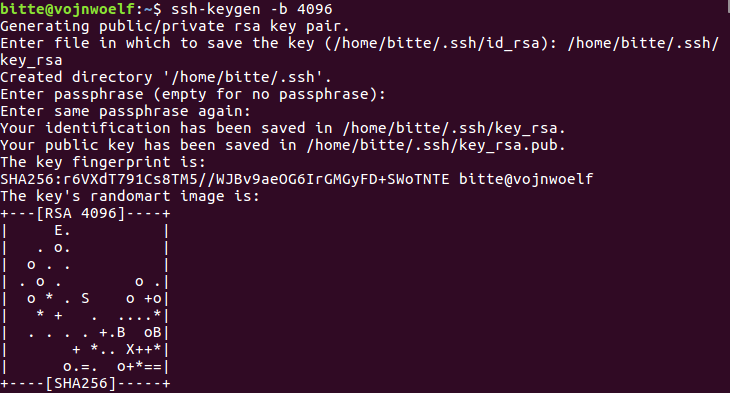
\includegraphics[width=0.8\linewidth]{images/generate_key}
	\figcaption{ssh-key wird generiert}
\end{minipage}


\subsubsection{Key auf Server übertragen}
Um den Key auf den Server zu übertragen, müssen Client und Server zuerst in einem Netzwerk sein. Dies wurde umgesetzt mit einem NAT-Netzwerk.

Der öffentliche Schlüssel wurde auf den Server kopiert mit:\\\verb|ssh-copy-id -i .ssh/key_rsa.pub bitte@10.0.2.6|

Es musste lediglich das Passwort des Benutzers am Server angegeben werden.

\begin{minipage}{\linewidth}
	\centering
	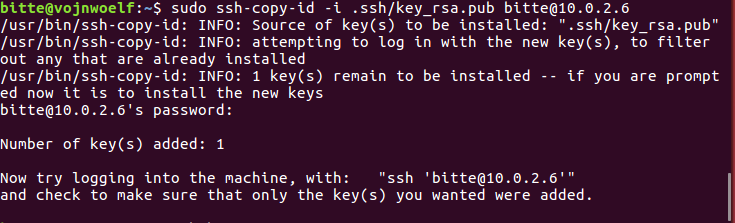
\includegraphics[width=0.8\linewidth]{images/transfer_key}
	\figcaption{Key wird auf Remote-Server übertragen}
\end{minipage}


\subsubsection{Auf server zugreifen}
Es kann sich nun am Server eingeloggt werden mit:\\\verb|ssh bitte@10.0.2.6|

Wichtig: Es wird nur mehr nach der Passphrase gefragt und nicht nach dem öffentlichen Schlüssel.

\begin{minipage}{\linewidth}
	\centering
	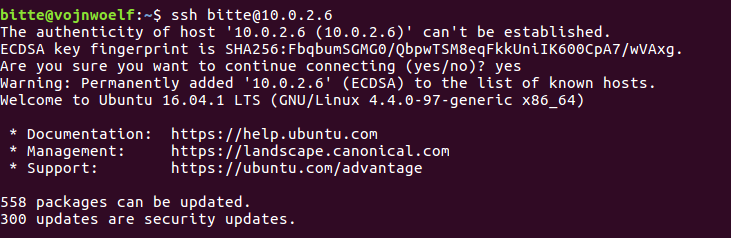
\includegraphics[width=0.8\linewidth]{images/access_server}
	\figcaption{Es wird auf den Server zugegriffen}
\end{minipage}

Auch zu beachten ist, nach dem ersten verbinden durch ssh wird auch nicht mehr nach der Passphrase gefragt.

\clearpage
\subsection{SSH-Tunnel Zugriff über Remote-Server}
\subsubsection{Server vorbereiten}
Um auf den Server über eine grafische Oberfläche zuzugreifen muss zuerst ein Desktop Environment und ein VNC-Server installiert werden.

\verb|sudo apt-get install xfce4 xfce4-goodies tightvncserver|

Nach der Installation wird der VNC-Server konfiguriert mit dem Befehl \verb|vncserver|:

\begin{minipage}{\linewidth}
	\centering
	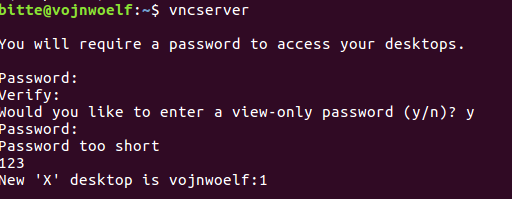
\includegraphics[width=0.8\linewidth]{images/vncserver}
	\figcaption{Der VNC-Server wird konfiguriert}
\end{minipage}

Tatsächlich wird nur nach einem Passwort für Remote Control (Tastatur und Maus) und View-Only definiert.

Nun soll noch geändert werden was passiert wenn ein VNC-Server gestartet wird. Dafür wird zuerst der service gekilled mit \verb|vncserver -kill :1|:

\begin{minipage}{\linewidth}
	\centering
	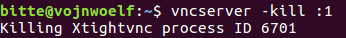
\includegraphics[width=0.8\linewidth]{images/kill_service}
	\figcaption{Der VNC-Server Service wird gekilled für Bearbeitung}
\end{minipage}

Anschließend wird das File geöffnet welches bestimmt welche Aktionen durchgeführt werden wenn der VNC-Server gestartet wird mit \verb|sudo nano ~/.vnc/xstartup|

Falls Inhalt bereits vorhanden ist, wird dieser aus dem File gelöscht, und folgender Inhalt wird hinzugefügt:

\begin{lstlisting}[language=bash]
#!/bin/bash
xrdb $HOME/.Xresources
startxfce4 &
\end{lstlisting}

Der Befehl \verb|xrdb $HOME/.Xresources| kümmert sich darum, dass der User bestimmte Einstellungen zu der grafischen Oberfläche machen kann wie Farben ändern, Designs oder Schriftarten.

Der zweite Befehl \verb|startxfce4 &| startet lediglich Xfce, was die komfortable Bearbeitung durch die grafische Oberfläche ermöglicht.


Es müssen diesem File auch noch bestimmte Privilegien zugewiesen werden: \\\verb|sudo chmod +x ~/.vnc/xstartup|

Der service kann nun durch \verb|vncserver| gestartet werden, der output sollte folgendermaßen aussehen:

\begin{minipage}{\linewidth}
	\centering
	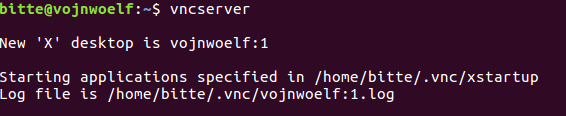
\includegraphics[width=0.8\linewidth]{images/start_service}
	\figcaption{Der VNC-Server wird wieder gestartet}
\end{minipage}

\subsubsection{Client vorbereiten}
In diesem Fall stellt die lokale Windows-Maschine den Client dar. Es werden 2 Programme benötigt, \verb|PuTTY| und \verb|TightVNC Viewer|.

Mit \verb|PuTTY| wird der SSH-Tunnel geöffnet und \verb|TightVNC Viewer| greift über diesen Tunnel auf die grafische Oberfläche des Servers zu.

\subsubsection{Mit Client zu Server verbinden}
Zuerst wird mit \verb|PuTTY| der Tunnel erstellt.

Dazu wird das Programm geöffnet und als IP-Adresse wird \verb|bitte@10.0.106.174| angegeben und es soll über SSH verbunden werden:

\begin{minipage}{\linewidth}
	\centering
	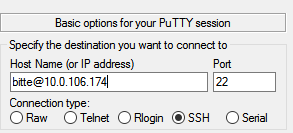
\includegraphics[width=0.8\linewidth]{images/user_ip}
	\figcaption{Es werden user, Ip-Adresse und Übertragungsart angegeben}
\end{minipage}

Der nächste Schritt ist es nun den Tunnel zu definieren. Diese Einstellung ist zu finden unter \verb|Connection|$\rightarrow$\verb|SSH|$\rightarrow$\verb|Tunnels|.

Hier wird als \verb|Source Port| ein beliebiger Port angegeben (Für das Beispiel wurde 9090 gewählt) und als \verb|Destination| wird der VNC-Server angegeben, mit der Adresse \verb|localhost:5901|. Es kann auf \verb|Add| gedrückt werden und man sollte folgendes Ergebnis sehen:

\begin{minipage}{\linewidth}
	\centering
	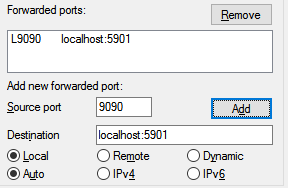
\includegraphics[width=0.8\linewidth]{images/ports}
	\figcaption{Es wurde ein Tunnel zum VNC Server hinzugefügt}
\end{minipage}

Nun kann auf \verb|Open| gedrückt werden und man sollte nach dem User-Passwort gefragt werden. Nach der Passworteingabe sollte man die Konsole des Servers sehen:

\begin{minipage}{\linewidth}
	\centering
	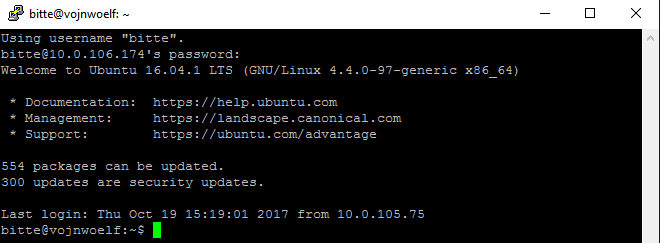
\includegraphics[width=0.8\linewidth]{images/console}
	\figcaption{Es wurde zum Server verbunden}
\end{minipage}

Das wichtige ist nun im \verb|Event Log| zu sehen, wenn man diesen öffnet (Rechtsklick auf Statusleiste$\rightarrow$Event Log) sollte man folgende 3 Zeilen sehen:

\begin{minipage}{\linewidth}
	\centering
	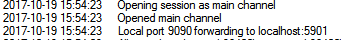
\includegraphics[width=0.8\linewidth]{images/event_log}
	\figcaption{Ein Channel mit Port forwarding zum Server wurde geöffnet}
\end{minipage}

Nun kann man den \verb|TightVNC Viewer| öffnen. Im Feld \verb|Remote Host| gibt man nun \verb|localhost:9090| an und wird wieder nach dem Passwort gefragt. Nach Eingabe des Passworts sollte die grafische Oberfläche des Server zu sehen sein:

\begin{minipage}{\linewidth}
	\centering
	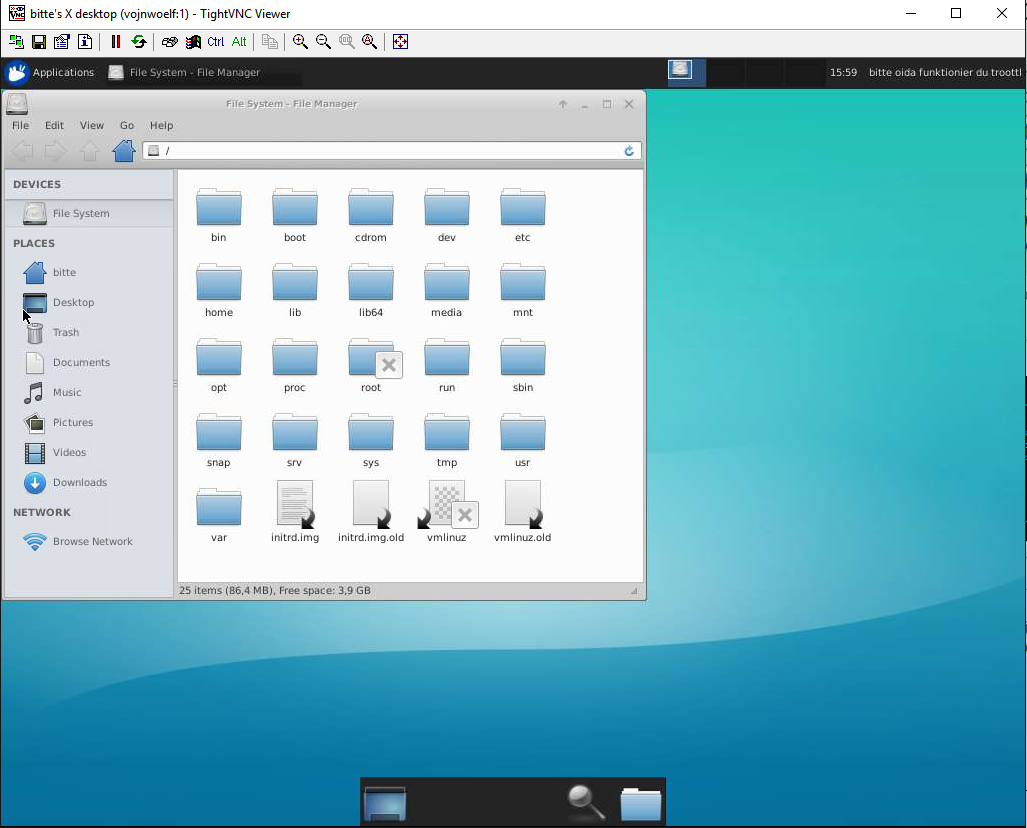
\includegraphics[width=0.8\linewidth]{images/gui}
	\figcaption{Es kann über eine grafische Oberfläche auf den Server zugegriffen werden}
\end{minipage}

Es wird nun mit dem Viewer auf den verschlüsselten SSH-Tunnel zugegriffen welcher eine Verbindung zum Server hat!
